\section{Timestamps}

Locking assumes collisions will occur, although in reality, collisions are infrequent.
Optimistic concurrency control methods like timestamps can be employed to address this. 
Timestamps are identifiers that establish a total ordering of a system's events. 
Each transaction is assigned a timestamp representing its initiation time, enabling transactions to be ordered based on their timestamps. 
A schedule is accepted only if it aligns with the serial ordering of transactions induced by their timestamps. 
Timestamps, given by a system's function upon request, have the syntax:
\[\left\langle \text{event-id}.\text{node-id} \right\rangle \]
The synchronization algorithm, known as the Lamport method, relies on the send-receive of messages. 
It ensures that a message from the future cannot be received. 
If this occurs, the bumping rule is employed to adjust the timestamp of the receiving event beyond that of the sending event.  
\begin{example}
    Timestamp assignment at two different nodes might look like the following.
    \begin{figure}[H]
        \centering
        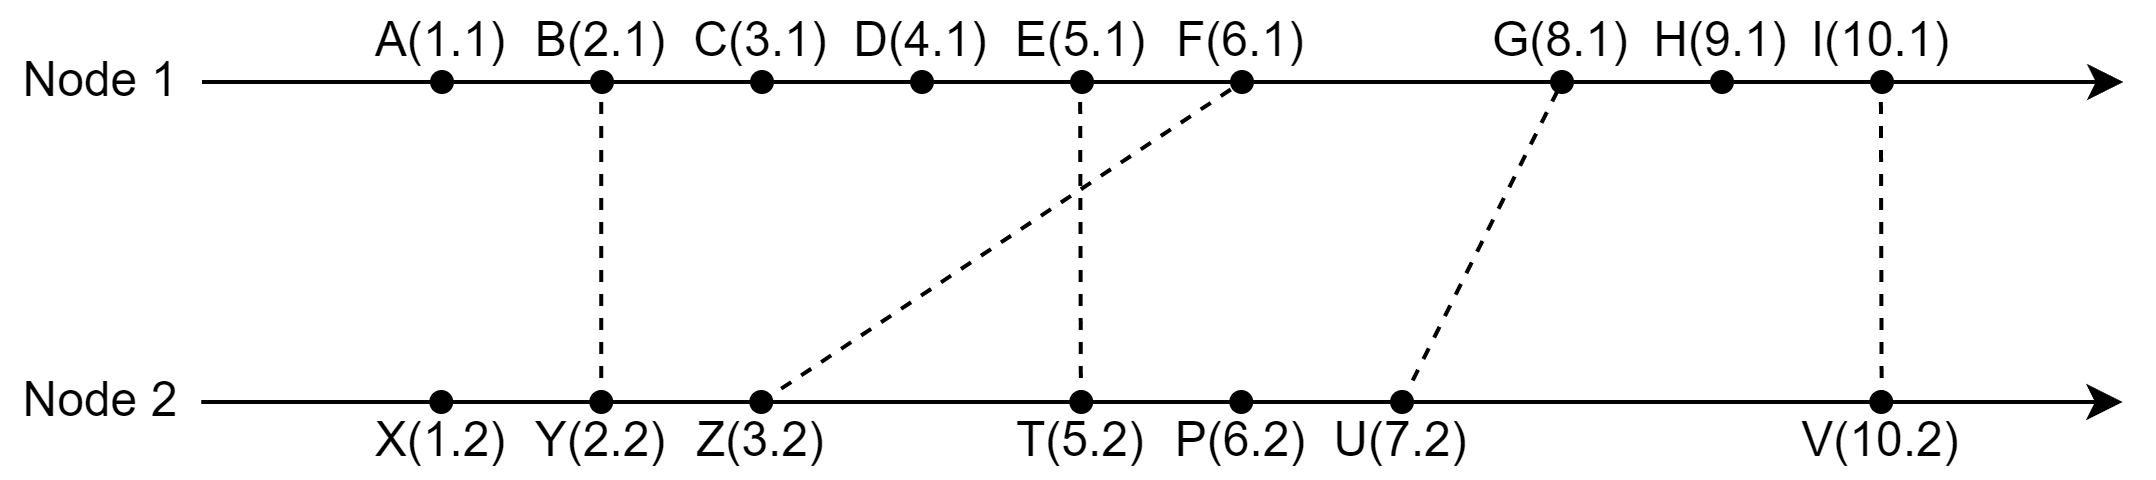
\includegraphics[width=0.75\linewidth]{images/timestamps.png}
    \end{figure}
\end{example}

\paragraph*{Counters}
The scheduler uses two counters: one for writes (WTM($x$)) and another for reads (RTM($x$)).
Read and write requests are tagged with the timestamp of the requesting transaction.

A read is accepted if its timestamp is higher than the last write timestamp.
In this case, $\text{RTM}(x)=\max(\text{RTM}(x),\text{ts})$. 

A write is accepted if its timestamp is higher than the last write and last read timestamps. 
In this case $\text{WTM}(x)=\text{ts}$. 

In case a read or a write is not accepted, the transaction is killed.
However, these rules may lead to excessive transaction killings.
\begin{example}
    Assuming $\text{RTM}(x)=7$ and $\text{WTM}(x)=4$, consider the following schedule:
    \[S=r_6(x) r_8(x) r_9(x) w_8(x) w_{11}(x) r_{10}(x)\]
    Using timestamps, we obtain:
    \begin{table}[H]
        \centering
        \begin{tabular}{ccc}
        \textbf{Request} & \textbf{Response} & \textbf{New value} \\ \hline
        $r_6(x)$         & $\checkmark$      & -                  \\
        $r_8(x)$         & $\checkmark$      & $\text{RTM}(x)=8$         \\
        $r_9(x)$         & $\checkmark$      & $\text{RTM}(x)=9$         \\
        $w_8(x)$         & $\tikzxmark$      & $T_8$ killed       \\
        $w_{11}(x)$      & $\checkmark$      & $\text{WTM}(x)=11$        \\
        $r_{10}(x)$      & $\tikzxmark$      & $T_{10}$ killed   
        \end{tabular}
    \end{table}
\end{example}
Comparing 2PL to is challenging, and there is no subset relationship between the two. 
However, TS implies CSR.
\begin{proof}
    Let $S$ be a TS schedule of $T_1$ and $T_2$. Suppose $S$ is not CSR, which implies that it contains a cycle between $T_1$ and $T_2$. 
    $S$ contains $op_1(x)$, $op_2(x)$ where at least one is a write. 
    $S$ contains also $op_2(y)$, $op_1(y)$ where at least one is a write. 
    When $op_1(y)$ arrives we have two possibilities. 
    If $op_1(y)$ is a read, $T_1$ is killed by TS because it tries to read a value written by a younger transaction, so it is a contradiction. 
    If $op_1(y)$ is a write, $T_1$ is killed no matter what $op_2(y)$ is, because it tries to write a value already read or written by a younger transaction, so it is a contradiction. 
\end{proof}

\paragraph*{Transaction abort}
Basic TS-based control considers only committed transactions, ignoring aborted transactions. 
If aborts occur, dirty reads may happen. 
To handle dirty reads, a variant of basic TS must be used. 
A transaction $T_i$ issuing $r_{\text{ts}}(x)$ or $w_{\text{ts}}(x)$ such that $\text{ts}>\text{WTM}(x)$ delays its read or write operation until the transaction $T^\prime$ that wrote the value of $x$ has committed or aborted. 
This is similar to long-duration write locks.
\begin{table}[H]
    \centering
    \begin{tabular}{c|cc}
    \textbf{Action} & \textbf{2PL}          & \textbf{TS}          \\ \hline
    Transaction     & Wait                  & Killed and restarted \\
    Serialization   & Imposed by conflicts  & Imposed by timestamp \\
    Delay           & Long (strict version) & Long                 \\
    Deadlocks       & Possible              & Prevented           
    \end{tabular}
\end{table}
Since restarting a transaction is costlier than waiting, 2PL is preferable when used alone. 
Commercial systems often combine these techniques to leverage the best features of both. 

\paragraph*{Thomas rule}
To reduce the number of killings, the Thomas rule can be used, altering the rule for write operations. 

A write is accepted if its timestamp is higher than the last read timestamp, and the write timestamp is updated. 
A write is skipped if its timestamp is lower than the last write timestamp. 

\subsection{Multi-version timestamp}
The concept of multi-versioning involves generating new versions with each write operation, and reads access the relevant version.
Each write produces new copies, each with a new write timestamp (WTM($x$)), ensuring that each object $x$ always has $N \geq 1$ active versions.
A unique global read timestamp (RTM($x$)) is maintained, and old versions are discarded when there are no transactions requiring their values.

The reads are always accepted and a copy $x_k$ is selected for reading, where:
\begin{itemize}
    \item If $\text{ts} \geq \text{WTM}_N(x)$, then $k=N$.
    \item Otherwise, $k$ is chosen such that $\text{WTM}_k(x) \leq \text{ts} < \text{WTM}_{k+1}(x)$. 
\end{itemize}
The write is accepted if its timestamp is higher than the last read timestamp, and the write timestamp is updated. 

\begin{example}
    Assuming  $\text{RTM}(x)=7$, $N=1$ and $\text{WTM}_1(x)=4$, consider the schedule:
    \[S=r_6(x) r_8(x) r_9(x) w_8(x) w_{11}(x) r_{10}(x) r_{12}(x) w_{14}(x) w_{13}(x)\]
    Using multi-versioning, the results are:
    \begin{table}[H]
        \centering
        \begin{tabular}{ccc}
        \textbf{Request} & \textbf{Response}         & \textbf{New value}  \\ \hline
        $r_6(x)$         & $\checkmark$              & -                   \\
        $r_8(x)$         & $\checkmark$              & $\text{RTM}(x)=8$          \\
        $r_9(x)$         & $\checkmark$              & $\text{RTM}(x)=9$          \\
        $w_8(x)$         & $\tikzxmark$              & $T_8$ killed        \\
        $w_{11}(x)$      & $\checkmark$              & $\text{WTM}_2(x)=11,\:N=2$ \\
        $r_{10}(x)$      & $\checkmark$ on $x_{(1)}$ & $\text{RTM}(x)=10$         \\
        $r_{12}(x)$      & $\checkmark$ on $x_{(2)}$ & $\text{RTM}(x)=12$         \\
        $w_{14}(x)$      & $\checkmark$              & $\text{WTM}_3(x)=14,\:N=3$ \\
        $w_{13}(x)$      & $\checkmark$              & $\text{WTM}_4(x)=14,\:N=4$
        \end{tabular}
    \end{table}
\end{example}

\paragraph*{Multi-versioning in practice}
In practice, the rule set is modified slightly.
The reads are always accepted and a copy $x_k$ is selected for reading, where:
\begin{itemize}
    \item If $\text{ts} \geq \text{WTM}_N(x)$, then $k=N$. 
    \item Otherwise, $k$ is chosen such that $\text{WTM}_k(x) \leq \text{ts} < \text{WTM}_{k+1}(x)$. 
\end{itemize}
The write is accepted if its timestamp is higher than the last read and last write timestamps, and the write timestamp is updated. 

\begin{example}
    Assuming $\text{RTM}(x)=7$, $N=1$ and $\text{WTM}_1(x)=4$, consider the schedule:
    \[S=r_6(x) r_8(x) r_9(x) w_8(x) w_{11}(x) r_{10}(x) r_{12}(x) w_{14}(x) w_{13}(x)\]
    Using multi-versioning, the results are:
    \begin{table}[H]
        \centering
        \begin{tabular}{ccc}
        \textbf{Request} & \textbf{Response}         & \textbf{New value}  \\ \hline
        $r_6(x)$         & $\checkmark$              & -                   \\
        $r_8(x)$         & $\checkmark$              & $\text{RTM}(x)=8$          \\
        $r_9(x)$         & $\checkmark$              & $\text{RTM}(x)=9$          \\
        $w_8(x)$         & $\tikzxmark$              & $T_8$ killed        \\
        $w_{11}(x)$      & $\checkmark$              & $\text{WTM}_2(x)=11,\:N=2$ \\
        $r_{10}(x)$      & $\checkmark$ on $x_{(1)}$ & $\text{RTM}(x)=10$         \\
        $r_{12}(x)$      & $\checkmark$ on $x_{(2)}$ & $\text{RTM}(x)=12$         \\
        $w_{14}(x)$      & $\checkmark$              & $\text{WTM}_3(x)=14,\:N=3$ \\
        $w_{13}(x)$      & $\tikzxmark$              & $T_{13}$ killed
        \end{tabular}
    \end{table}
\end{example}

\paragraph*{Isolation levels}
The implementation of TS-multi opens the door to introducing another isolation level in the DBMS (DBMS), known as snapshot isolation.
In this level, only Write Timestamp (WTM($x$)) is utilized.
The rule applied in snapshot isolation dictates that every transaction reads the version consistent with its timestamp and defers writes until the end. 
If the scheduler detects conflicts between the writes of a transaction and the writes of other concurrent transactions after the snapshot timestamp, it aborts.
It's essential to note that while snapshot isolation provides certain guarantees, it does not ensure serializability, and a new anomaly known as write skew (non-determinism) can occur.